\chapter{Marco teorico}
\section{Marco Conceptual}

% \subsection{Lectura aumentada y realidad aumentada espacial}

%Se entiende por \textbf{lectura aumentada} el enriquecimiento de un documento impreso con prestaciones propias del formato digital (búsqueda, definición, traducción, anotación sincronizada) sin reemplazar el papel como soporte de lectura. Cuando la información digital se dibuja directamente sobre los objetos físicos mediante un proyector, en lugar de mostrarse en una pantalla o un visor que el usuario sostiene o lleva puesto, se habla de \textbf{realidad aumentada espacial} \citep{bimber2005}. Esta modalidad es \textbf{no obstructiva}: el lector no necesita sostener un dispositivo ni llevar un casco, lo que la hace adecuada para estudiar la lectura sin alterar la conducta que se quiere medir.

%Un sistema de este tipo necesita relacionar tres sistemas de coordenadas: el de la cámara que observa el escritorio, el de la imagen del proyector y el del documento PDF. La relación entre dos planos observados en perspectiva se modela con una \textbf{homografía}, una transformación proyectiva $H \in \mathbb{R}^{3\times3}$ que lleva un punto homogéneo $p=(x,y,1)^\top$ de un plano a otro, $p' \sim Hp$, y que puede estimarse con al menos cuatro pares de puntos correspondientes \citep{hartley2004}. En EDDIE la homografía se obtiene de una calibración de cuatro puntos y permite convertir la posición de un lápiz o de un dedo en la cámara en una posición sobre la proyección.

%\subsection{Percepción del documento: binarización y OCR}

%La \textbf{binarización} separa los píxeles de tinta de los del fondo. El método de \citet{otsu1979} elige el umbral $t^\ast$ que maximiza la varianza entre las dos clases del histograma de grises,
%\begin{equation}
%t^\ast=\arg\max_{t}\ \omega_0(t)\,\omega_1(t)\,\bigl[\mu_0(t)-\mu_1(t)\bigr]^2,
%\end{equation}
%donde $\omega_i$ y $\mu_i$ son la proporción y la media de cada clase. Es un umbral \emph{global}: un único valor para toda la imagen, por lo que se degrada cuando la iluminación no es uniforme, como ocurre con la luz de un proyector sobre papel. Los umbrales \emph{adaptativos} calculan un valor por vecindad y toleran mejor esos gradientes.

%El \textbf{reconocimiento óptico de caracteres} (OCR) convierte la imagen de un texto en una cadena de caracteres. EDDIE usa el motor Tesseract \citep{smith2007}. Su calidad se mide con la tasa de error por carácter (CER) y por palabra (WER), que cuentan las sustituciones ($S$), supresiones ($D$) e inserciones ($I$) necesarias para transformar la transcripción en el texto de referencia de largo $N$, es decir, su distancia de edición de \citet{levenshtein1966}:
%\begin{equation}
%\mathrm{CER}=\frac{S_c+D_c+I_c}{N_c}\times100\%,\qquad
%\mathrm{WER}=\frac{S_w+D_w+I_w}{N_w}\times100\%.
%\end{equation}

%\subsection{Rastreo ocular e interacción por la mirada}

%Un \textbf{eye tracker} estima, a una frecuencia de muestreo fija (60~Hz en GazePoint y TheEyeTribe), el punto de la escena al que mira una persona. La señal se compone de \textbf{fijaciones}, períodos en que la mirada permanece estable sobre una región y en los que se procesa la información, y \textbf{sacadas}, desplazamientos rápidos entre fijaciones. Un método habitual para identificar fijaciones es el de dispersión (I-DT), que agrupa muestras consecutivas mientras su dispersión no supere un umbral durante un tiempo mínimo \citep{salvucci2000}.

%Cuando la mirada se usa además para \emph{actuar} (seleccionar un botón), el sistema debe distinguir entre mirar para leer y mirar para activar. El \textbf{clic por permanencia} (\textit{dwell time}) dispara la acción cuando la mirada permanece dentro de un radio $R$ durante un tiempo $T$. Si $T$ es corto, cualquier fijación de lectura activa controles involuntariamente, problema conocido como \textbf{toque de Midas} \citep{jacob1990}; si es largo, la interacción se vuelve lenta. La elección de $(T,R)$ es, por lo tanto, un compromiso que debe medirse.

%\subsection{Software científico y deuda técnica}

%En este trabajo se entiende por \textbf{software científico} aquel desarrollado \textit{ad hoc} para soportar una tarea de investigación específica, como la captura, el procesamiento o el análisis de datos experimentales, en contraposición al software de propósito general que un laboratorio utiliza como herramienta auxiliar. Bajo esta definición, EDDIE y Multimodal Observer son software científico, mientras que el sistema operativo o el editor de código empleados en su desarrollo no lo son.

%La \textbf{deuda técnica} es el costo futuro que generan las decisiones de diseño o implementación que resuelven un problema inmediato a expensas de la mantenibilidad. En el software científico aparece con frecuencia porque cada investigador optimiza para su propio trabajo y no para el sistema común \citep{ernst2026}.

%\subsection{Arquitectura de plugins y orquestación}

%Una \textbf{arquitectura de plugins} separa un núcleo estable de módulos intercambiables que implementan un \textbf{contrato de interfaz} común, de modo que se puede agregar o reemplazar un módulo sin modificar el núcleo \citep{bustio2013}. El \textbf{orquestador} es el componente del núcleo que conoce a todos los plugins, controla su ciclo de vida (inicialización, ejecución y liberación) y coordina el flujo de datos entre ellos, a diferencia de un esquema de coreografía en que los módulos se coordinan entre sí sin un componente central \citep{megargel2021}. Una \textbf{capa de abstracción de hardware} (HAL) oculta detrás de una interfaz los detalles de cada dispositivo físico, lo que permite sustituirlo por una implementación simulada para pruebas.

%\subsection{MECIVA PS}

%\textbf{MECIVA PS} es la metodología de evaluación y validación de software científico aplicada por \citet{ibaceta2023evaluacion} a EDDIE. Clasifica los requisitos en críticos y secundarios, ejecuta verificaciones funcionales y no funcionales, registra los errores encontrados con su estado (sin falla, solución parcial, sin solución) y evalúa la validez y la confiabilidad de las mediciones del sistema mediante ejecuciones repetidas. En este trabajo se usa como protocolo de verificación del sistema reconstruido, de modo que sus resultados sean comparables con la línea base de 2023 (Capítulo~\ref{cap:evaluacion}).



\section{Estado del arte}
\subsection{Antecedentes del Proyecto (Evolución Histórica)}
Para comprender los fundamentos sobre los que se sustenta la presente propuesta de modernización, es necesario reconstruir la trayectoria histórica del sistema EDDIE (Entorno Digital y Dinámico de Interacción Escrita), desarrollado de forma incremental en el Departamento de Ingeniería Informática de la Universidad de Santiago de Chile bajo el alero del laboratorio InTeractiOn. El proyecto constituye un caso representativo de software científico que ha evolucionado orgánicamente a través de seis memorias de título sucesivas, cada una incorporando un nuevo módulo funcional sin que existiera, en ningún momento del proceso, una revisión sistemática de la arquitectura común subyacente.

El concepto original fue propuesto por \cite{carrasco2017diseno}, quien implementó un entorno de realidad aumentada móvil orientado a enriquecer la lectura en papel mediante dispositivos portátiles. \cite{contreras2019desarrollo} evolucionó esta propuesta hacia una configuración no obstructiva de escritorio, sustituyendo el dispositivo móvil por un sistema fijo de cámara y proyector que elimina la necesidad de mediadores físicos manuales. A partir de esta base, el proyecto se expandió mediante la incorporación sucesiva de tres capacidades de soporte al lector: \cite{montanares2019desarrollo} integró un módulo de búsqueda web contextual activado por voz y gestos; \cite{pezoa2020implementacion} desarrolló un mecanismo de consistencia bidireccional entre el documento físico y su versión digital en PDF; y \cite{estay2020integracion} incorporó dispositivos de rastreo ocular (eye-tracking) para el análisis del comportamiento atencional del usuario. Posteriormente, \cite{santibanez2020rediseno} realizó un rediseño de la interfaz gráfica bajo un enfoque centrado en el usuario, y finalmente \cite{ibaceta2023evaluacion} aplicó la metodología MECIVA PS para diagnosticar cuantitativamente el estado del software, identificando 67 errores estructurales acumulados a lo largo de este proceso de crecimiento.

\begin{table}[htbp]
    \centering
    \caption{Síntesis de la evolución histórica del sistema EDDIE a través de seis memorias de título sucesivas.}
    \label{tab:evolucion_eddie}
    \small
    \begin{tabularx}{\textwidth}{|>{\raggedright\arraybackslash}p{3.0cm}|>{\raggedright\arraybackslash}X|>{\raggedright\arraybackslash}X|}
        \hline
        \textbf{Trabajo / Investigador} & \textbf{Aporte al proyecto EDDIE} & \textbf{Limitaciones / Deuda técnica generada} \\ \hline
        \cite{carrasco2017diseno} & Prototipo inicial de lectura aumentada en dispositivos móviles. & Dependencia de mediadores manuales (pantalla móvil). \\ \hline
        \cite{contreras2019desarrollo} & Configuración no obstructiva de escritorio (cámara + proyector). & Acoplamiento directo con la interfaz WinForms en C\#. \\ \hline
        \cite{montanares2019desarrollo} & Módulo de búsqueda web contextual (Wikipedia, diccionarios). & Carga mediante reflexión con \texttt{Assembly.LoadFile}. \\ \hline
        \cite{pezoa2020implementacion} & Módulo de consistencia bidireccional físico-digital (PDF). & Incompatibilidades de sincronización y fallo por rutas fijas. \\ \hline
        \cite{estay2020integracion} & Integración de rastreo ocular (eye-tracking). & Carga aislada por Proxy Sandbox en \texttt{AppDomain} subordinado. \\ \hline
        \cite{santibanez2020rediseno} & Rediseño centrado en el usuario de la interfaz gráfica. & Mantenimiento de la capa monolítica subyacente. \\ \hline
        \cite{ibaceta2023evaluacion} & Diagnóstico cuantitativo de errores mediante metodología MECIVA PS. & Revelación de 67 errores estructurales por falta de validación en hardware real. \\ \hline
    \end{tabularx}
    \fuente{Elaboración propia a partir de \cite{carrasco2017diseno}, \cite{contreras2019desarrollo}, \cite{montanares2019desarrollo}, \cite{pezoa2020implementacion}, \cite{estay2020integracion}, \cite{santibanez2020rediseno} e \cite{ibaceta2023evaluacion}.}
\end{table}

Este proceso incremental produjo un sistema monolítico de aproximadamente 45.000 líneas de código distribuidas en 26 proyectos .csproj, en el cual la falta de una arquitectura común provocó la coexistencia de tres mecanismos heterogéneos de carga por reflexión (Assembly.LoadFrom, AppDomain Proxy Sandbox y Assembly.LoadFile), origen directo de más de 30 de los 67 errores documentados por \cite{ibaceta2023evaluacion}.

\subsubsection{Catálogo de funcionalidades y levantamiento de la usabilidad previa}
En su estado actual, EDDIE ofrece cinco categorías funcionales heredadas directamente de las memorias descritas: procesamiento de imágenes y reconocimiento gestual \citep{contreras2019desarrollo}, búsqueda web contextual \citep{montanares2019desarrollo}, consistencia bidireccional entre el documento físico y su versión digital \citep{pezoa2020implementacion}, rastreo ocular \citep{estay2020integracion}, y una capa de presentación en WinForms resultante del rediseño centrado en el usuario de \cite{santibanez2020rediseno}. Cada una de estas funcionalidades fue incorporada mediante un mecanismo de integración propio del memorista responsable, sin que se estableciera en ningún caso un contrato de interfaz común entre ellas, lo cual explica la heterogeneidad de mecanismos de carga identificada posteriormente en el diagnóstico del sistema. 

El levantamiento de usabilidad realizado por \cite{ibaceta2023evaluacion} mediante la metodología MECIVA PS constituye el diagnóstico más completo disponible sobre el estado funcional de EDDIE previo a esta propuesta. Su evaluación identificó fallas tanto internas (relacionadas con la consistencia de los módulos entre sí) como externas, vinculadas a la interacción del sistema con el hardware físico y a la ausencia de documentación de uso e instalación. Entre los hallazgos más críticos se cuentan fallas no resueltas en la conexión con hardware, como la inestabilidad de la cámara digital (error E16) y la imposibilidad de detectar zonas de la proyección mediante el eyetracker (error E49), lo que compromete directamente la validez de EDDIE como instrumento de medición científica del comportamiento atencional. Este diagnóstico funcional constituye la línea base contra la cual se contrastaron los resultados de la reconstrucción propuesta en este trabajo.

% Ajusta los espacios de las subsecciones: {left}{before-spacing}{after-spacing}
\titlespacing{\subsection}{0pt}{*1.0}{*0.5}
\subsection{Sistemas de lectura aumentada similares}

El proyecto EDDIE no existe en un vacío tecnológico, por lo que existen tanto sistemas de lectura aumentada comparables, como plataformas de software que han enfrentado problemáticas de modernización arquitectónicas. Entre los referentes más destacados se encuentran:

\begin{itemize}
\item \textbf{DigitalDesk:} Este sistema pionero introdujo el concepto de "Entorno Aumentado por Computadora", utilizando una arquitectura basada en cámaras de video y un proyector electrónico montados sobre un escritorio físico convencional. Su objetivo es dotar a los documentos de papel de propiedades electrónicas y viceversa. Entre sus aplicaciones destacan una calculadora interactiva que permite al usuario señalar números impresos en un informe para ingresarlos automáticamente mediante OCR, un sistema de traducción que proyecta definiciones de palabras extranjeras directamente sobre el escritorio, y PaperPaint, una herramienta que permite seleccionar bocetos hechos a mano en papel y "pegarlos" como objetos digitales proyectados.
\end{itemize}

\begin{figure}[H]
    \centering
    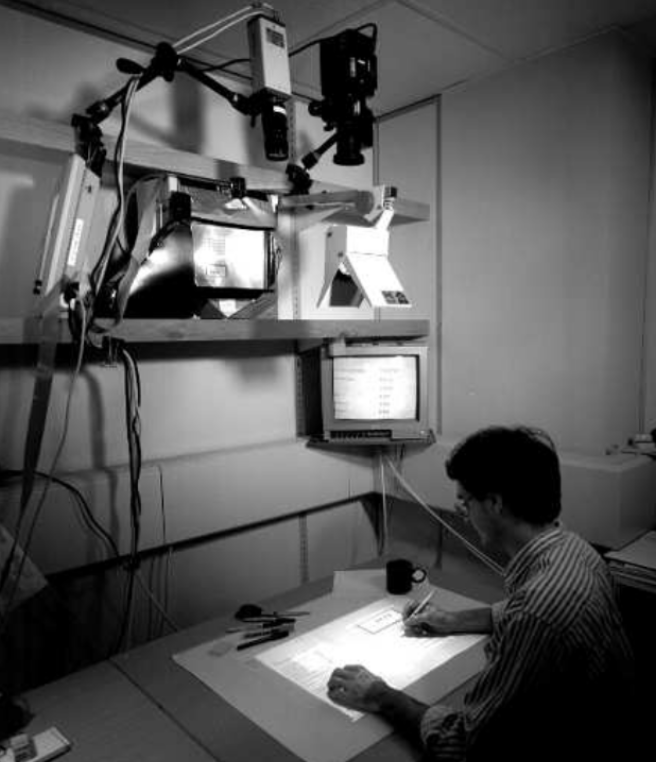
\includegraphics[width=0.40\textwidth]{images/digitaldesk.png}
    \caption{El primer prototipo de DigitalDesk.}
    \label{fig:digitaldesk}
    \fuente{Wellner, P. (1993). Interacting with paper on the DigitalDesk. \textit{Communications of the ACM}, 36(7), 87--96. \url{https://doi.org/10.1145/159544.159630}}
\end{figure}
\vspace{0.3cm} % Espacio antes del siguiente punto

\begin{itemize}
    \item \textbf{EnhancedDesk:} Evoluciona la idea del escritorio aumentado resolviendo problemas críticos de visión artificial, como la sensibilidad a la iluminación. Arquitectónicamente, incorpora una cámara infrarroja que detecta el calor corporal para realizar un seguimiento de los dedos en tiempo real (25-30 cuadros por segundo) de manera robusta, sin importar los colores proyectados sobre la piel. Su aplicación principal es el "Interactive Textbook", donde códigos de matriz 2D en las páginas de un libro físico activan simulaciones digitales dinámicas (como experimentos de física de resortes o péndulos) que el estudiante puede manipular directamente con sus manos.
\end{itemize}

\begin{figure}[H]
    \centering
    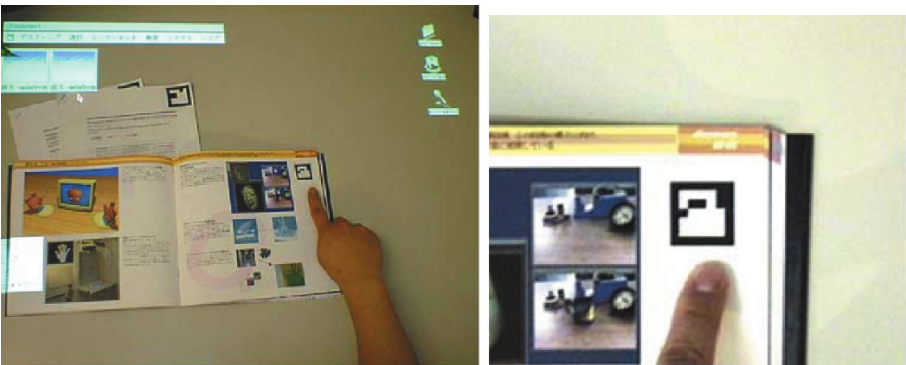
\includegraphics[width=0.65\textwidth]{images/enhanceddesk.png}
    \caption{Gesto de señalamiento del usuario para EnhancedDesk.}
    \label{fig:enhanceddesk}
    \fuente{Koike, H., Sato, Y., \& Kobayashi, Y. (2001). Integrating paper and digital information on EnhancedDesk: A method for real-time finger tracking on an augmented desk system. ACM Transactions on Computer-Human Interaction, 8(4), 307–322. \url{https://doi.org/10.1145/504704.504706}}
\end{figure}

\begin{itemize}
    \item \textbf{AR-PaperSync:} Es un sistema de Realidad Aumentada móvil que busca la integración perfecta entre documentos científicos físicos y digitales. Permite a los investigadores escanear el título de un artículo impreso para visualizar instantáneamente capas de información con citas interactivas y referencias guardadas. Su arquitectura soporta la sincronización en tiempo real de notas de lectura entre dispositivos móviles, aplicaciones de escritorio y el papel físico, reduciendo significativamente la carga cognitiva y mejorando la eficiencia en la navegación de literatura académica.
\end{itemize}

\begin{figure}[H]
    \centering
    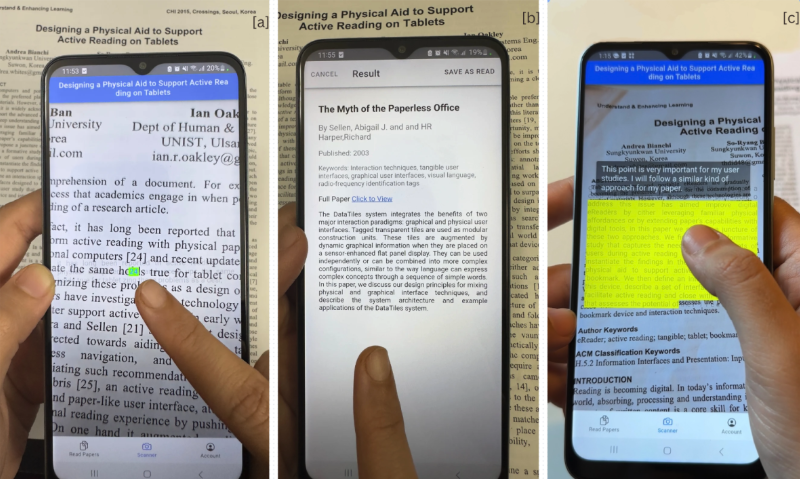
\includegraphics[width=0.55\textwidth]{images/arpapersync.png}
    \caption{Descripción general de AR-PaperSync.}
    \label{fig:arpapersync}
    \vspace{0.2cm}
    \small
    \centering
    \textit{Fuente: agregar agregar agregar agregar agregar aaaaaaaaaaaaaaaaaaaggggggggggrrrrrreeeeeeeeggggggarrrr} . \url{https://doi.org/10.1145/504704.504706}
\end{figure}

\begin{itemize}
    \item \textbf{Enlight:} Es una lámpara de escritorio inteligente que utiliza visión computacional, reconocimiento óptico de caracteres, conexión a fuentes de datos en red y tecnología de projection-mapping para traer funciones inteligentes a libros impresos y documentos de cualquier época. Los usuarios pueden subrayar palabras para ver definiciones; si se resalta un pasaje, el sistema provee definiciones enciclopédicas contextuales, estadísticas de WolframAlpha y otros datos. Los highlights se sincronizan con la nube y pueden verse en otros dispositivos. A diferencia de EDDIE, es un prototipo conceptual de diseño de interacción (proyecto de grado MFA) sin módulos de eye-tracking ni consistencia bidireccional, pero comparte el mismo principio de proyección no obstructiva sobre el libro físico.
\end{itemize}

\begin{figure}[H]
    \centering
    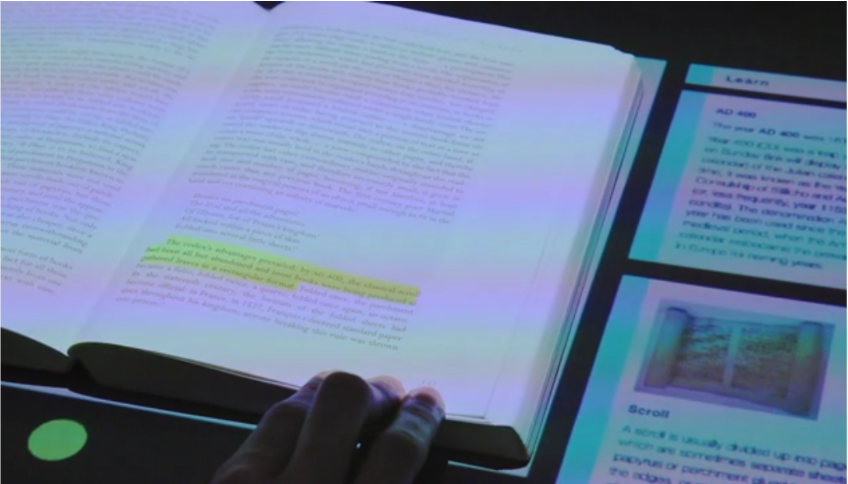
\includegraphics[width=0.65\textwidth]{images/enlight.png}
    \caption{Enlight: Lectura Aumentada.}
    \label{fig:enlight}
    \fuente{. \url{https://doi.org/10.1145/504704.504706}}
\end{figure}

\begin{table}[htbp]
    \centering
    \caption{Comparación de sistemas.}
    \label{tab:comparacion_sistemas}
    \small
    \begin{tabularx}{\textwidth}{|>{\raggedright\arraybackslash}X|c|c|c|c|}
        \hline
        \textbf{Sistema} & \textbf{Proyección} & \textbf{Eye} & \textbf{Consistencia} & \textbf{Foco} \\
        & \textbf{sobre papel} & \textbf{tracking} & \textbf{bidireccional} & \textbf{académico} \\ \hline
        EDDIE & Sí & Sí & Sí & Sí \\ \hline
        DigitalDesk & Sí & No & Parcial & No \\ \hline
        EnhancedDesk & Sí & No & No & Sí \\ \hline
        AR-PaperSync & No (Móvil) & No & Sí & Sí \\ \hline
        enlight & Sí & No & Parcial & Sí \\ \hline
    \end{tabularx}
    \fuente{Elaboración propia.}
\end{table}

\subsection{El problema de la modernización en software de investigación}
En este trabajo se entiende por software científico aquel desarrollado ad hoc para soportar una tarea de investigación específica, como la captura, procesamiento o análisis de datos experimentales, en contraposición al software de propósito general que un laboratorio pueda utilizar como herramienta auxiliar (sistemas operativos, editores de texto, suites ofimáticas). Bajo esta definición, EDDIE y MO son software científico, mientras que el sistema operativo o el editor de código empleados durante su desarrollo no lo son, dado que no fueron construidos para responder a un problema de investigación particular. 

Un desafío documentado en el desarrollo de este tipo de software es que decisiones técnicas localmente óptimas (las que son tomadas por un investigador para resolver el problema inmediato de su propia tesis) tienden a resultar en un sistema globalmente inconsistente cuando se acumulan a través de múltiples autores sin una arquitectura común \citep{ernst2026nature}. Este fenómeno ha sido documentado en sistemas de mayor escala, como plataformas de bioinformática y biología computacional, donde la falta de coordinación entre grupos de desarrollo genera herramientas difíciles de integrar entre sí \citep{orozco2017diseno}. La literatura converge en que la solución recurrente a este problema es la adopción de arquitecturas modulares con interfaces estandarizadas que separan la lógica de investigación de la infraestructura técnica subyacente \citep{bustio2013arquitectura,glatard2017software}. En el dominio específico de los science gateways (plataformas que integran instrumentos y flujos de trabajo científicos), esta separación se implementa habitualmente mediante una capa de abstracción de hardware y un catálogo de plugins cargados dinámicamente a través de un único mecanismo, lo que permite aislar el fallo de un componente sin comprometer el resto del sistema \citep{glatard2017software}. Esta misma arquitectura de núcleo liviano con contratos de interfaz bien definidos es la que permite minimizar el tiempo dedicado a resolver problemas comunes de integración, concentrando el esfuerzo de desarrollo en la implementación de los algoritmos propios de cada dominio de investigación \citep{bustio2013arquitectura}.

\subsection{Multimodal Observer (MO) como referente arquitectural}
Un hito crítico para la propuesta actual es la evolución del MO, una aplicación del mismo laboratorio InTeractiOn diseñada para la captura y análisis de datos multimodales como movimientos oculares, bioseñales y video. MO enfrentó un problema estructuralmente idéntico al de EDDIE: las sucesivas versiones de su núcleo, desarrolladas por distintos tesistas para incorporar nuevos módulos, generaron incompatibilidades que dejaron la mayoría de sus plugins de visualización y análisis inoperativos en las versiones más recientes. La solución adoptada fue una re-implementación completa del núcleo en Python con una arquitectura de plugins desacoplada, la cual demostró ser viable en el contexto académico y produjo un sistema validado con métricas objetivas de calidad de código, rendimiento y aceptación \citep{figueroa2025arquitectura}. Esta experiencia constituye el antecedente empírico más relevante para la presente propuesta, tanto por la similitud estructural del problema como por compartir el mismo contexto institucional y línea de investigación.

\begin{figure}[H]
    \centering
    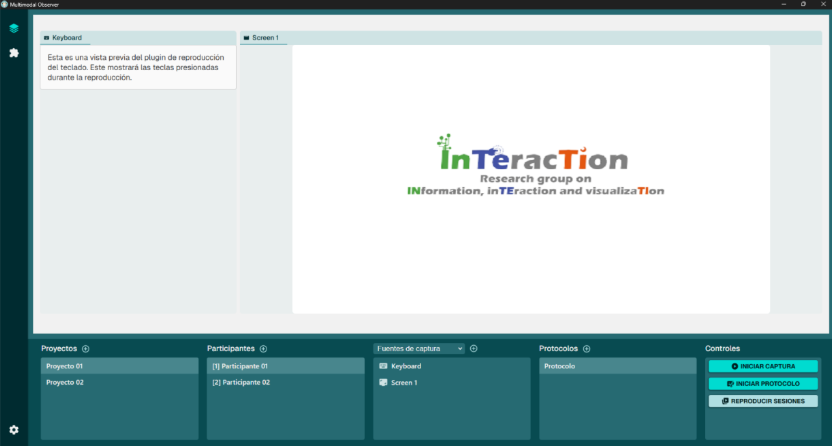
\includegraphics[width=0.65\textwidth]{images/mo.png}
    \caption{Multimodal Observer (MO) - Vista principal.}
    \label{fig:mo}
    \vspace{0.2cm}
    \small
    \centering
    \textit{Fuente: Contreras, M. F. (2025). Arquitectura basada en plugins para la captura y análisis de datos
multimodales: El caso de Multimodal Observer . Memoria de título, Universidad de Santiago
de Chile.} 
\end{figure}